% Options for packages loaded elsewhere
\PassOptionsToPackage{unicode}{hyperref}
\PassOptionsToPackage{hyphens}{url}
%
\documentclass[
]{article}
\usepackage{amsmath,amssymb}
\usepackage{iftex}
\ifPDFTeX
  \usepackage[T1]{fontenc}
  \usepackage[utf8]{inputenc}
  \usepackage{textcomp} % provide euro and other symbols
\else % if luatex or xetex
  \usepackage{unicode-math} % this also loads fontspec
  \defaultfontfeatures{Scale=MatchLowercase}
  \defaultfontfeatures[\rmfamily]{Ligatures=TeX,Scale=1}
\fi
\usepackage{lmodern}
\ifPDFTeX\else
  % xetex/luatex font selection
\fi
% Use upquote if available, for straight quotes in verbatim environments
\IfFileExists{upquote.sty}{\usepackage{upquote}}{}
\IfFileExists{microtype.sty}{% use microtype if available
  \usepackage[]{microtype}
  \UseMicrotypeSet[protrusion]{basicmath} % disable protrusion for tt fonts
}{}
\makeatletter
\@ifundefined{KOMAClassName}{% if non-KOMA class
  \IfFileExists{parskip.sty}{%
    \usepackage{parskip}
  }{% else
    \setlength{\parindent}{0pt}
    \setlength{\parskip}{6pt plus 2pt minus 1pt}}
}{% if KOMA class
  \KOMAoptions{parskip=half}}
\makeatother
\usepackage{xcolor}
\usepackage[margin=1in]{geometry}
\usepackage{color}
\usepackage{fancyvrb}
\newcommand{\VerbBar}{|}
\newcommand{\VERB}{\Verb[commandchars=\\\{\}]}
\DefineVerbatimEnvironment{Highlighting}{Verbatim}{commandchars=\\\{\}}
% Add ',fontsize=\small' for more characters per line
\usepackage{framed}
\definecolor{shadecolor}{RGB}{248,248,248}
\newenvironment{Shaded}{\begin{snugshade}}{\end{snugshade}}
\newcommand{\AlertTok}[1]{\textcolor[rgb]{0.94,0.16,0.16}{#1}}
\newcommand{\AnnotationTok}[1]{\textcolor[rgb]{0.56,0.35,0.01}{\textbf{\textit{#1}}}}
\newcommand{\AttributeTok}[1]{\textcolor[rgb]{0.13,0.29,0.53}{#1}}
\newcommand{\BaseNTok}[1]{\textcolor[rgb]{0.00,0.00,0.81}{#1}}
\newcommand{\BuiltInTok}[1]{#1}
\newcommand{\CharTok}[1]{\textcolor[rgb]{0.31,0.60,0.02}{#1}}
\newcommand{\CommentTok}[1]{\textcolor[rgb]{0.56,0.35,0.01}{\textit{#1}}}
\newcommand{\CommentVarTok}[1]{\textcolor[rgb]{0.56,0.35,0.01}{\textbf{\textit{#1}}}}
\newcommand{\ConstantTok}[1]{\textcolor[rgb]{0.56,0.35,0.01}{#1}}
\newcommand{\ControlFlowTok}[1]{\textcolor[rgb]{0.13,0.29,0.53}{\textbf{#1}}}
\newcommand{\DataTypeTok}[1]{\textcolor[rgb]{0.13,0.29,0.53}{#1}}
\newcommand{\DecValTok}[1]{\textcolor[rgb]{0.00,0.00,0.81}{#1}}
\newcommand{\DocumentationTok}[1]{\textcolor[rgb]{0.56,0.35,0.01}{\textbf{\textit{#1}}}}
\newcommand{\ErrorTok}[1]{\textcolor[rgb]{0.64,0.00,0.00}{\textbf{#1}}}
\newcommand{\ExtensionTok}[1]{#1}
\newcommand{\FloatTok}[1]{\textcolor[rgb]{0.00,0.00,0.81}{#1}}
\newcommand{\FunctionTok}[1]{\textcolor[rgb]{0.13,0.29,0.53}{\textbf{#1}}}
\newcommand{\ImportTok}[1]{#1}
\newcommand{\InformationTok}[1]{\textcolor[rgb]{0.56,0.35,0.01}{\textbf{\textit{#1}}}}
\newcommand{\KeywordTok}[1]{\textcolor[rgb]{0.13,0.29,0.53}{\textbf{#1}}}
\newcommand{\NormalTok}[1]{#1}
\newcommand{\OperatorTok}[1]{\textcolor[rgb]{0.81,0.36,0.00}{\textbf{#1}}}
\newcommand{\OtherTok}[1]{\textcolor[rgb]{0.56,0.35,0.01}{#1}}
\newcommand{\PreprocessorTok}[1]{\textcolor[rgb]{0.56,0.35,0.01}{\textit{#1}}}
\newcommand{\RegionMarkerTok}[1]{#1}
\newcommand{\SpecialCharTok}[1]{\textcolor[rgb]{0.81,0.36,0.00}{\textbf{#1}}}
\newcommand{\SpecialStringTok}[1]{\textcolor[rgb]{0.31,0.60,0.02}{#1}}
\newcommand{\StringTok}[1]{\textcolor[rgb]{0.31,0.60,0.02}{#1}}
\newcommand{\VariableTok}[1]{\textcolor[rgb]{0.00,0.00,0.00}{#1}}
\newcommand{\VerbatimStringTok}[1]{\textcolor[rgb]{0.31,0.60,0.02}{#1}}
\newcommand{\WarningTok}[1]{\textcolor[rgb]{0.56,0.35,0.01}{\textbf{\textit{#1}}}}
\usepackage{longtable,booktabs,array}
\usepackage{calc} % for calculating minipage widths
% Correct order of tables after \paragraph or \subparagraph
\usepackage{etoolbox}
\makeatletter
\patchcmd\longtable{\par}{\if@noskipsec\mbox{}\fi\par}{}{}
\makeatother
% Allow footnotes in longtable head/foot
\IfFileExists{footnotehyper.sty}{\usepackage{footnotehyper}}{\usepackage{footnote}}
\makesavenoteenv{longtable}
\usepackage{graphicx}
\makeatletter
\def\maxwidth{\ifdim\Gin@nat@width>\linewidth\linewidth\else\Gin@nat@width\fi}
\def\maxheight{\ifdim\Gin@nat@height>\textheight\textheight\else\Gin@nat@height\fi}
\makeatother
% Scale images if necessary, so that they will not overflow the page
% margins by default, and it is still possible to overwrite the defaults
% using explicit options in \includegraphics[width, height, ...]{}
\setkeys{Gin}{width=\maxwidth,height=\maxheight,keepaspectratio}
% Set default figure placement to htbp
\makeatletter
\def\fps@figure{htbp}
\makeatother
\setlength{\emergencystretch}{3em} % prevent overfull lines
\providecommand{\tightlist}{%
  \setlength{\itemsep}{0pt}\setlength{\parskip}{0pt}}
\setcounter{secnumdepth}{5}
\usepackage{booktabs}
\usepackage{longtable}
\usepackage{array}
\usepackage{multirow}
\usepackage{wrapfig}
\usepackage{float}
\usepackage{colortbl}
\usepackage{pdflscape}
\usepackage{tabu}
\usepackage{threeparttable}
\usepackage{threeparttablex}
\usepackage[normalem]{ulem}
\usepackage{makecell}
\usepackage{xcolor}
\usepackage{siunitx}

  \newcolumntype{d}{S[
    input-open-uncertainty=,
    input-close-uncertainty=,
    parse-numbers = false,
    table-align-text-pre=false,
    table-align-text-post=false
  ]}
  
\ifLuaTeX
  \usepackage{selnolig}  % disable illegal ligatures
\fi
\IfFileExists{bookmark.sty}{\usepackage{bookmark}}{\usepackage{hyperref}}
\IfFileExists{xurl.sty}{\usepackage{xurl}}{} % add URL line breaks if available
\urlstyle{same}
\hypersetup{
  pdftitle={Does protected area connectivity moderate the efficacy of protection on tropical biodiversity? Evidence from a replication of Brodie et al.~2023},
  pdfauthor={Peter Kedron, Lei Song, Wenxin Yang, Amy Frazier},
  hidelinks,
  pdfcreator={LaTeX via pandoc}}

\title{Does protected area connectivity moderate the efficacy of
protection on tropical biodiversity? Evidence from a replication of
Brodie et al.~2023}
\author{Peter Kedron, Lei Song, Wenxin Yang, Amy Frazier}
\date{2024-02-14}

\begin{document}
\maketitle

\hypertarget{abstract}{%
\section*{Abstract}\label{abstract}}
\addcontentsline{toc}{section}{Abstract}

This study is a \emph{reproduction} of:

\begin{quote}
Brodie, J.F., Mohd-Azlan, J., Chen, C. et al.~Landscape-scale benefits
of protected areas for tropical biodiversity. Nature 620, 807--812
(2023). \url{https://doi.org/10.1038/s41586-023-06410-z}
\end{quote}

We replicate the analysis of Brodie et al.~(2023) and introduce
protected area (PA) connectivity as a statistical moderator of the
effect PA status has on biodiversity. We find KEY FINDINGS. Using a
causal framework that controls for forest structure, site accessibility,
and geographic location through matching, Brodie et al.~(2023) find
evidence that protected areas (PA) do preserve vertebrate biodiversity
within their boundaries and in the adjacent unprotected landscape.
Brodie et al.~provides evidence of the efficacy of protected area
status, they do not assess whether the effect they observe is altered by
network connectivity.

\hypertarget{study-metadata}{%
\section{Study metadata}\label{study-metadata}}

This replication uses the data file provided by Brodie et al.~(2023) at
\url{https://doi.org/10.6084/m9.figshare.22527298.v1}. We independently
accessed the World Database on Protected Areas
\url{https://www.protectedplanet.net/en/thematic-areas/wdpa?tab=WDPA} to
construct our site and PA connectivity measures.

\begin{itemize}
\tightlist
\item
  \texttt{Key\ words}: Biodiversity, Conservation, Protected Areas,
  Connectivity, 30x30
\item
  \texttt{Subject}: Ecology and Evolutionary Biology, Natural Resources
  and Conservation,
\item
  \texttt{Date\ created}: November 8, 2023
\item
  \texttt{Date\ modified}: date of most recent revision
\item
  \texttt{Spatial\ Coverage}: Southeast Asia
\item
  \texttt{Spatial\ Resolution}: Species observations - GPS located point
  data, GEDI-derived forest structural covariates - 1 km raster, HDI -
  country-level, Protected Areas - PA Polygons
\item
  \texttt{Spatial\ Reference\ System}: Specify the geographic or
  projected coordinate system for the study, e.g.~EPSG:4326
\item
  \texttt{Temporal\ Coverage}: 01-2015 to 08-2021
\item
  \texttt{Temporal\ Resolution}: Specify the temporal resolution of your
  study---i.e.~the duration of time for which each observation
  represents or the revisit period for repeated observations
\end{itemize}

\hypertarget{study-design}{%
\section{Study design}\label{study-design}}

This study consists of a reproduction of the original work by Brodie et
al.~(2023) and a replication to analyze how connectivity influences
protected area efficacy in preserving tropical biodiversity. We first
implement the workflow as described and shared in Brodie et al.~(2023)
as identically as possible to reproduce the original study. We then
compute and add connectivity measures at the sample points to the
original dataset to further examine the effect of connectivity.

Brodie et al.~(2023) formulated hypotheses to assess protected area
effectiveness and tested them with structural causal modeling.
Hypotheses concerned overall protected area effectiveness (H1) and PAs'
size (H2) and closeness (H3) effects on biodiversity in unprotected
lands to infer implications for spillover and leakage effects.

\hypertarget{protected-area-effectiveness-on-overall-biodiversity}{%
\subsection{Protected area effectiveness on overall
biodiversity}\label{protected-area-effectiveness-on-overall-biodiversity}}

\begin{quote}
OR-H1: Biodiversity is higher within protected areas than outside (after
removing effects of site accessbility and habitat condition).
\end{quote}

Debates exist on whether protected areas are effective because of their
remote location and good habitat conditions or conservation status
itself. Motivated by such, Brodie et al.~(2023) estimated protected
areas efficacy for conserving tropical mammal and bird diversity after
de-confounding the effects of site accessibility and habitat condition
(H1). Their outcome variables are various aspects of biodiversity. The
treatment variable is whether the observation point is within or outside
a reserve. If the treatment variable is significant in a causal model,
it supports H1 and adds evidence for the effectiveness of protecting
lands.

To do so, they removed confounding effects and built causal models for
birds vs mammals, and different biodiversity outcome metrics. Two major
confounders identified were site accessibility and habitat quality. Site
accessibility was proxied using Human Development Index (HDI), circuit
theory-based measures of proximity to human development\footnote{``circuit
  theoretical models parameterized with human travel speeds across
  different terrains and the locations of populations centers and
  transportation networks'' (Brodie et al.~2023)}, and an interaction
term of the two variables. Habitat quality was proxied using
three-dimensional habitat structure metrics derived from the Global
Ecosystem Dynamics Investigation (GEDI) mission. Confounding effects
were removed using statistical matching based on propensity scores.
Biodiversity metrics used as outcome variables include species richness
(SR), functional richness (FR), and phylogenetic diversity (PD). PA
effects were estimated using separate mixed effects linear regression
for different biodiversity metrics and for birds vs mammals.

Brodie et al.~(2023) found protection status increased all facets of
bird biodiversity but the effects were not significant for mammals.

\hypertarget{spillover-and-leakage-effects-on-unprotected-lands}{%
\subsection{Spillover and leakage effects on unprotected
lands}\label{spillover-and-leakage-effects-on-unprotected-lands}}

Spillover and leakage effects are two ways protected areas could have
regional impacts on biodiversity beyond their boundaries. Spillover
effect refers to enhanced biodiversity in unprotected lands near PAs
whereas leakage effect refers to increased conservation pressure (e.g.,
unregulated hunting and displaced disturbances) in nearby unprotected
lands because of PA establishment. Brodie et al.~(2023) tested the
effects of PA sizes (H2) and closeness (i.e., distance, H3) to
neighboring unprotected lands.

\begin{quote}
OR-H2: Biodiversity outside protected areas is higher when they are near
large ones (size effect).
\end{quote}

They built separate models for birds and mammals on three different
diversity metrics and tested H2 using observations outside protected
areas. They went through the same matching steps as above.

Brodie et al.~(2023) found that PA size is a significant predictor of
all facets of birds and mammals diversity outside PAs in the study
region. Effects for mammals were smaller than those for birds.

\begin{quote}
OR-H3: Biodiversity outside protected areas is higher when they are
closer (distance effect).
\end{quote}

They tested the effect of proximity to PAs on biodiversity outside PAs.
Distance was computed as the Euclidean distance to the nearest reserve.

In the original paper, the authors reported that no significant effects
of distance were observed. However, regression summary for H3 was
incomplete in Extended Data Table 1 so that a direct comparison could
not be made.

\hypertarget{adding-connectivity}{%
\subsection{Adding connectivity}\label{adding-connectivity}}

We ask the research question of whether protected areas moderate the
efficacy of protection on tropical biodiversity. We formulate the
hypothesis is as follows:

\begin{quote}
RPL-H1: Connectivity mdoerates the efficacy of protection on
biodiversity.
\end{quote}

We build upon the existing structural causal models by Brodie et
al.~(2023) to test the hypothesis. The original study archetype is
quasi-experimental as it uses a matching strategy to perform causal
analysis.

\hypertarget{materials-and-procedure}{%
\section{Materials and procedure}\label{materials-and-procedure}}

\hypertarget{computational-environment}{%
\subsection{Computational environment}\label{computational-environment}}

The reproduction of the original study is conducted in MacBook Pros.
Brodie et al.~(2023) cleaned up the variables and performed propensity
score matching and causal analysis in R. They did not provide scripts on
how they derived the biodiversity metrics, circuit theory-based metrics,
HDI, and the GEDI metrics. We built upon and annotated R scripts shared
by the original study, and added missing information on HDI and GEDI
metrics to the scripts. // Is this accurate?

Required packages are as follows:

\begin{Shaded}
\begin{Highlighting}[]
\CommentTok{\# library(groundhog)}
\NormalTok{pkgs }\OtherTok{\textless{}{-}} \FunctionTok{c}\NormalTok{(}\StringTok{"tidyverse"}\NormalTok{, }\StringTok{"cowplot"}\NormalTok{, }\StringTok{"here"}\NormalTok{, }\StringTok{"dagitty"}\NormalTok{, }\StringTok{"ggdag"}\NormalTok{, }\StringTok{"Hmisc"}\NormalTok{, }
          \StringTok{"MatchIt"}\NormalTok{, }\StringTok{"modelsummary"}\NormalTok{, }\StringTok{"optmatch"}\NormalTok{, }\StringTok{"nlme"}\NormalTok{)}
\CommentTok{\# groundhog.library(pkgs, "2024{-}02{-}11")}
\CommentTok{\# I don\textquotesingle{}t know why groundhog is not working}
\FunctionTok{lapply}\NormalTok{(pkgs, require, }\AttributeTok{character.only=}\ConstantTok{TRUE}\NormalTok{)}
\end{Highlighting}
\end{Shaded}

\hypertarget{data-and-variables}{%
\subsection{Data and variables}\label{data-and-variables}}

In the original study, outcome variables for the causal models are
biodiversity metrics (i.e., species richness, functional richness, and
phylogenetic diversity) derived from species observations. Mammal
observations were assembled by the authors from camera traps in 65 study
areas in the study region. Bird observations were gathered from eBird
from 2015/01 to 2021/08 following a set of filtering procedures.

Treatment variables for ORIG-H1, H2, H3 were derived from the World
Database on Protected Areas (WDPA) by UNEP-WCMC. Specifically, they are
1) a binary variable on whether the sampling point is within protected
areas or not (H1), 2) relative size of the closest protected area (i.e.,
large or small, H2), and 3) euclidean distance to the closest protected
area (H3). For H2, PAs equal to or larger than 500 km2 are considered
large and otherwise small. The size threshold was determined by testing
a series of values with the best model fits for birds and mammals
(Extended Data Table 4 in Brodie et al.~2023).

Observations were matched based on propoensity scores of their
geographic locations (i.e., latitudes and longitudes), forest canopy
height, accessibility, and HDI. Predictors in the mixed-effects linear
regression models were forest canopy height, site accessibility, HDI,
and treatment variables.

We gathered data shared by Brodie et al.~(2023). Tabular data of most
model inputs were provided in a
\href{https://doi.org/10.6084/m9.figshare.22527298.v1}{figshare}. Raster
files at 1-km resolution for GEDI derived metrics and circuit-based
accessibility were shared through a
\href{https://rcdata.nau.edu/geode_data/SEA_vertebrate_diversity_rasters}{weblink}.
Variable sources are presented in Table 1.

\emph{Table 1}. Variables used in Brodie et al.~(2023)

\begin{longtable}[]{@{}
  >{\centering\arraybackslash}p{(\columnwidth - 4\tabcolsep) * \real{0.3333}}
  >{\centering\arraybackslash}p{(\columnwidth - 4\tabcolsep) * \real{0.3333}}
  >{\centering\arraybackslash}p{(\columnwidth - 4\tabcolsep) * \real{0.3333}}@{}}
\toprule\noalign{}
\begin{minipage}[b]{\linewidth}\centering
\textbf{Name}
\end{minipage} & \begin{minipage}[b]{\linewidth}\centering
\textbf{Source}
\end{minipage} & \begin{minipage}[b]{\linewidth}\centering
\textbf{Usage}
\end{minipage} \\
\midrule\noalign{}
\endhead
\bottomrule\noalign{}
\endlastfoot
Biodiversity metrics - mammals & Authors & Outcome variable (ORIG-H1,
H2, H3) \\
Biodiversity metrics - birds & eBird & Outcome variable (ORIG-H1, H2,
H3) \\
Protected area boundaries & WDPA & Treatment variables (whether inside
PAs: ORIG-H1, distance to PAs: ORIG-H2, and size of PAs: ORIG-H3) \\
Ground elevation & NASA GEDI L2B & Predictor - elevation and
topography \\
Circuit-based site accessibility (log transformed) & Authors & Predictor
- site accessibility \\
Human Development Index & Human Development Report 2020 & Predictor -
site accessibility \\
Forest structure metrics & NASA GEDI L2A & Predictor - forest
structure \\
\end{longtable}

\hypertarget{ebird}{%
\subsubsection{eBird}\label{ebird}}

The original study gathered bird observations from eBird.

\begin{itemize}
\tightlist
\item
  \texttt{Title}: eBird.
\item
  \texttt{Abstract}: A community science platform for reporting bird
  sightings.
\item
  \texttt{Spatial\ Coverage}: Tropical region (overlapping countries of
  Brunei, Cambodie, China, Indonesia, Laos, Malaysia, Singapore,
  Thailand, and Vietnam).
\item
  \texttt{Spatial\ Resolution}: Vector.
\item
  \texttt{Spatial\ Reference\ System}: Not specified.
\item
  \texttt{Temporal\ Coverage}: 2015/01 - 2021/08.
\item
  \texttt{Temporal\ Resolution}: Not applicable.
\item
  \texttt{Lineage}: Brodie et al.~(2023) queried and subset data
  directly from eBird website or its R package or API.
\item
  \texttt{Distribution}: \href{https://ebird.org/home}{eBird webpage}
  and
  \href{https://science.ebird.org/en/use-ebird-data/download-ebird-data-products}{other
  download methods}.
\item
  \texttt{Constraints}: Non-commercial use.
\item
  \texttt{Data\ Quality}: Although a direct data quality layer is not
  associated, Brodie et al.~(2023) followed recommendations from
  existing studies to filter out data points.
\end{itemize}

Variables constructed were as follows:

\emph{Table 2} Variables created from bird observations via eBird.

\begin{longtable}[]{@{}
  >{\centering\arraybackslash}p{(\columnwidth - 14\tabcolsep) * \real{0.1250}}
  >{\centering\arraybackslash}p{(\columnwidth - 14\tabcolsep) * \real{0.1250}}
  >{\centering\arraybackslash}p{(\columnwidth - 14\tabcolsep) * \real{0.1250}}
  >{\centering\arraybackslash}p{(\columnwidth - 14\tabcolsep) * \real{0.1250}}
  >{\centering\arraybackslash}p{(\columnwidth - 14\tabcolsep) * \real{0.1250}}
  >{\centering\arraybackslash}p{(\columnwidth - 14\tabcolsep) * \real{0.1250}}
  >{\centering\arraybackslash}p{(\columnwidth - 14\tabcolsep) * \real{0.1250}}
  >{\centering\arraybackslash}p{(\columnwidth - 14\tabcolsep) * \real{0.1250}}@{}}
\toprule\noalign{}
\begin{minipage}[b]{\linewidth}\centering
\textbf{Label}
\end{minipage} & \begin{minipage}[b]{\linewidth}\centering
\textbf{Alias}
\end{minipage} & \begin{minipage}[b]{\linewidth}\centering
\textbf{Definition}
\end{minipage} & \begin{minipage}[b]{\linewidth}\centering
\textbf{Type}
\end{minipage} & \begin{minipage}[b]{\linewidth}\centering
\textbf{Accuracy}
\end{minipage} & \begin{minipage}[b]{\linewidth}\centering
\textbf{Domain}
\end{minipage} & \begin{minipage}[b]{\linewidth}\centering
\textbf{Missing Data Value(s)}
\end{minipage} & \begin{minipage}[b]{\linewidth}\centering
\textbf{Missing Data Frequency}
\end{minipage} \\
\midrule\noalign{}
\endhead
\bottomrule\noalign{}
\endlastfoot
SR.mean & Species richness & Number of species & Float & Unknown & Equal
or greater than 0 & Not applicable & Unknown \\
maxFRic & Functional richness & Diversity of species functional traits &
Float & Unknown & Equal or greater than 0 & Not applicable & Unknown \\
asymptPD & Phylogenetic diversity & Cumulative evolutionary time of the
species assemblage & Float & Unknown & Equal or greater than 0 & Not
applicable & Unknown \\
\end{longtable}

\hypertarget{the-world-database-on-protected-areas}{%
\subsubsection{The World Database on Protected
Areas}\label{the-world-database-on-protected-areas}}

The original study used protected area boundaries to derive the three
treatment variables (Table 3). Brodie et al.~(2023) did not specify how
they cleaned up protected area boundary. We dissolved PAs and then
converted them from multi-parts to single-parts to avoid double
counting. For mammals, we excluded marine protected areas.

// need to confirm with Lei.

\begin{itemize}
\tightlist
\item
  \texttt{Title}: The World Database on Protected Areas (WDPA).
\item
  \texttt{Abstract}: A global database on protected areas (PAs) and
  other effective conservation measurers (OECM).
\item
  \texttt{Spatial\ Coverage}: Tropical region (overlapping countries of
  Brunei, Cambodie, China, Indonesia, Laos, Malaysia, Singapore,
  Thailand, and Vietnam).
\item
  \texttt{Spatial\ Resolution}: Vector.
\item
  \texttt{Spatial\ Reference\ System}: WGS 84.
\item
  \texttt{Temporal\ Coverage}: Latest.
\item
  \texttt{Temporal\ Resolution}: Updated monthly.
\item
  \texttt{Lineage}: Brodie et al.~(2023) queried and subset data
  directly from eBird website or its R package or API.
\item
  \texttt{Distribution}:
  \href{https://www.protectedplanet.net/en/thematic-areas/wdpa?tab=WDPA}{WDPA
  webpage}.
\item
  \texttt{Constraints}: Non-commercial use.
\item
  \texttt{Data\ Quality}: Unknown.
\end{itemize}

\emph{Table 3} Variables created from protected area boundaries.

\begin{longtable}[]{@{}
  >{\centering\arraybackslash}p{(\columnwidth - 14\tabcolsep) * \real{0.1250}}
  >{\centering\arraybackslash}p{(\columnwidth - 14\tabcolsep) * \real{0.1250}}
  >{\centering\arraybackslash}p{(\columnwidth - 14\tabcolsep) * \real{0.1250}}
  >{\centering\arraybackslash}p{(\columnwidth - 14\tabcolsep) * \real{0.1250}}
  >{\centering\arraybackslash}p{(\columnwidth - 14\tabcolsep) * \real{0.1250}}
  >{\centering\arraybackslash}p{(\columnwidth - 14\tabcolsep) * \real{0.1250}}
  >{\centering\arraybackslash}p{(\columnwidth - 14\tabcolsep) * \real{0.1250}}
  >{\centering\arraybackslash}p{(\columnwidth - 14\tabcolsep) * \real{0.1250}}@{}}
\toprule\noalign{}
\begin{minipage}[b]{\linewidth}\centering
\textbf{Label}
\end{minipage} & \begin{minipage}[b]{\linewidth}\centering
\textbf{Alias}
\end{minipage} & \begin{minipage}[b]{\linewidth}\centering
\textbf{Definition}
\end{minipage} & \begin{minipage}[b]{\linewidth}\centering
\textbf{Type}
\end{minipage} & \begin{minipage}[b]{\linewidth}\centering
\textbf{Accuracy}
\end{minipage} & \begin{minipage}[b]{\linewidth}\centering
\textbf{Domain}
\end{minipage} & \begin{minipage}[b]{\linewidth}\centering
\textbf{Missing Data Value(s)}
\end{minipage} & \begin{minipage}[b]{\linewidth}\centering
\textbf{Missing Data Frequency}
\end{minipage} \\
\midrule\noalign{}
\endhead
\bottomrule\noalign{}
\endlastfoot
PA & Within or outside PAs & Whether the point is inside a PA or not &
Binary & Not applicable & 1 for inside and 0 for outside & Not
applicable & Unknown \\
PA\_size\_km2 & Functional richness & Diversity of species functional
traits & Float & Unknown & Equal or greater than 0 & Not applicable &
Unknown \\
dist\_to\_PA & Phylogenetic diversity & Cumulative evolutionary time of
the species assemblage & Float & Unknown & Equal or greater than 0 & Not
applicable & Unknown \\
\end{longtable}

\hypertarget{gedi-l2-metrics}{%
\subsubsection{GEDI L2 metrics}\label{gedi-l2-metrics}}

The Global Ecosystem Dynamics Investigation (GEDI) is a spaceborne light
detection and ranging (LiDAR) mission monitoring forest structure on
earth. The original study derived both ground elevation and forest
structure metrics from the Level 2 dataset of GEDI. Level 2 GEDI data
are at footprint level so Brodie et al.~(2023) used krigging
interpolation to create wall-to-wall layers (1-km resolution).

L2A includes elevation data. The original study computed slope and
topographic position index (TPI) to represent topographic traits at each
site. The original study used five L2B metrics, which were canopy height
(relative height at 95\%), plant area volume density (PAVD) between 0
and 5 m (represents understory density), cumulative plant area index
from ground to canopy top, foliage height diversity of plant area index,
and proportional cover. They found the five forest structure metrics to
be highly correlated and only kept canopy height and understory density
in models.

\begin{itemize}
\tightlist
\item
  \texttt{Title}: The Global Ecosystem Dynamics Investigation Level 2
  Elevation and Height Metrics.
\item
  \texttt{Abstract}: Global footprint level observations from GEDI on
  ground elevation and forest structure.
\item
  \texttt{Spatial\ Coverage}: Tropical region (overlapping countries of
  Brunei, Cambodie, China, Indonesia, Laos, Malaysia, Singapore,
  Thailand, and Vietnam).
\item
  \texttt{Spatial\ Resolution}: Footprints are of 25-m resolution and
  extrapolated into 1-km resolution.
\item
  \texttt{Spatial\ Reference\ System}: WGS 84.
\item
  \texttt{Temporal\ Coverage}: 2019/04/17 to 2022/04/12
\item
  \texttt{Temporal\ Resolution}: Not applicable.
\item
  \texttt{Lineage}: Brodie et al.~(2023) queried and subset data
  directly from eBird website or its R package or API.
\item
  \texttt{Distribution}: Original GEDI L2 metrics can be derived from
  \href{https://cmr.earthdata.nasa.gov/search/concepts/C1908348134-LPDAAC_ECS.html}{NASA
  website} and Brodie et al.~(2023) shared krigged results on a
  \href{https://rcdata.nau.edu/geode_data/SEA_vertebrate_diversity_rasters}{webpage}.
\item
  \texttt{Constraints}: Non-commercial use.
\item
  \texttt{Data\ Quality}: Original GEDI L2 metrics have quality and
  degrade flags and Brodie et al.~(2023) kept only data points of
  satisfying quality.
\end{itemize}

\emph{Table 4} Variables derived from GEDI L2 metrics.

\begin{longtable}[]{@{}
  >{\centering\arraybackslash}p{(\columnwidth - 14\tabcolsep) * \real{0.1250}}
  >{\centering\arraybackslash}p{(\columnwidth - 14\tabcolsep) * \real{0.1250}}
  >{\centering\arraybackslash}p{(\columnwidth - 14\tabcolsep) * \real{0.1250}}
  >{\centering\arraybackslash}p{(\columnwidth - 14\tabcolsep) * \real{0.1250}}
  >{\centering\arraybackslash}p{(\columnwidth - 14\tabcolsep) * \real{0.1250}}
  >{\centering\arraybackslash}p{(\columnwidth - 14\tabcolsep) * \real{0.1250}}
  >{\centering\arraybackslash}p{(\columnwidth - 14\tabcolsep) * \real{0.1250}}
  >{\centering\arraybackslash}p{(\columnwidth - 14\tabcolsep) * \real{0.1250}}@{}}
\toprule\noalign{}
\begin{minipage}[b]{\linewidth}\centering
\textbf{Label}
\end{minipage} & \begin{minipage}[b]{\linewidth}\centering
\textbf{Alias}
\end{minipage} & \begin{minipage}[b]{\linewidth}\centering
\textbf{Definition}
\end{minipage} & \begin{minipage}[b]{\linewidth}\centering
\textbf{Type}
\end{minipage} & \begin{minipage}[b]{\linewidth}\centering
\textbf{Accuracy}
\end{minipage} & \begin{minipage}[b]{\linewidth}\centering
\textbf{Domain}
\end{minipage} & \begin{minipage}[b]{\linewidth}\centering
\textbf{Missing Data Value(s)}
\end{minipage} & \begin{minipage}[b]{\linewidth}\centering
\textbf{Missing Data Frequency}
\end{minipage} \\
\midrule\noalign{}
\endhead
\bottomrule\noalign{}
\endlastfoot
elev & Elevation & Ground elevation at the site (krigged) & Integer &
Unknown & Equal to or greater than 0 (terrestrial observations) &
Unknown & Unknown \\
slope & Slope & Slope of topography & Float & Unknown & 0 to 90 &
Unknown & Unknown \\
TPI & Topographic Position Index & Difference between the elevation of a
focal raster cell with those of its neighbors (not mentioned in paper) &
Float & Unknwon & Not bounded & Unknown & Unknown \\
rh\_95\_a0.pred & Relative height at 95\% & Roughly the top canopy
height (krigged) & Float & Unknown & Equal to or greater than 0 &
Unknown & Unknown \\
pavd\_0\_5.pred & Plant area volume density from 0 to 5 m & A proxy of
understory forest density (krigged) & Float & Unknown & Equal to or
greater than 0 & Unknown & Unknown \\
pai\_a0.pred & Plant area index & Cumulative PAI from ground to canopy
(krigged) & Float & Unknown & Equal to or greater than 0 & Unknown &
Unknown \\
fhd\_pai\_1m\_a0.pred & Foliage height diversity & Shannon's diversity
of PAI across heights (krigged) & Float & Unknown & Equal to or greater
than 0 & Unknown & Unknown \\
cover\_a0.pred & Proportional coverage & Openness or closeness of canopy
(krigged) & Float & Unknown & 0 to 1 & Unknown & Unknown \\
\end{longtable}

\hypertarget{human-development-index-hdi}{%
\subsubsection{Human Development Index
(HDI)}\label{human-development-index-hdi}}

Human Development Index for each country was included in the causal
models as a simple metric of socioeconomic level.

\begin{itemize}
\item
  \texttt{Title}: Human Development Index
\item
  \texttt{Abstract}: An index on the level of human development by
  country.
\item
  \texttt{Spatial\ Coverage}: Tropical region (overlapping countries of
  Brunei, Cambodie, China, Indonesia, Laos, Malaysia, Singapore,
  Thailand, and Vietnam).
\item
  \texttt{Spatial\ Resolution}: Not applicable.
\item
  \texttt{Spatial\ Reference\ System}: Not applicable.
\item
  \texttt{Temporal\ Coverage}: 2020.
\item
  \texttt{Temporal\ Resolution}: Not applicable.
\item
  \texttt{Lineage}: Direct query thourgh the official website.
\item
  \texttt{Distribution}: Acquired directly through
  \href{https://hdr.undp.org/sites/default/files/2021-22_HDR/HDR21-22_Statistical_Annex_HDI_Table.xlsx}{Human
  Development Report 2020}.
\item
  \texttt{Constraints}: Non-commercial use.
\item
  \texttt{Data\ Quality}: Unknown.
\item
  \texttt{Variables}: HDI

  \begin{itemize}
  \tightlist
  \item
    \texttt{Label}: Not included in the files shared by the original
    study, we added HDI values and labeled as `HDI'.
  \item
    \texttt{Alias}: Human Development Index
  \item
    \texttt{Definition}: A metric on the level of human development.
  \item
    \texttt{Type}: Float
  \item
    \texttt{Accuracy}: Unknown
  \item
    \texttt{Domain}: 0 to 1
  \item
    \texttt{Missing\ Data\ Value(s)}: Not applicable
  \item
    \texttt{Missing\ Data\ Frequency}: Not applicable
  \end{itemize}
\end{itemize}

\hypertarget{prior-observations}{%
\subsection{Prior observations}\label{prior-observations}}

At the beginning of this analysis, we had observed the dataset provided
by Brodie et al with their publication. We noticed the following caveats
in the script and raw data shared by the original study. 1) HDI was
missing. 2) The process of variable construction for biodiversity
metrics and GEDI metrics were unclear. 3) The procedure for
preprocessing and cleaning PA boundaries was unclear.

We did not manipulate the data before beginning our reproduction
attempt.

\hypertarget{bias-and-threats-to-validity}{%
\subsection{Bias and threats to
validity}\label{bias-and-threats-to-validity}}

Given the research design and primary data to be collected and/or
secondary data to be used, discuss common threats to validity and the
approach to mitigating those threats, with an emphasis on geographic
threats to validity.

Given the research design as described in the original paper and primary
data shared, we identify potential spatial autocorrelation of sample
points were not addressed. // should we add a map/moran's I result here?
// other concerns to add?

These include: - uneven primary data collection due to geographic
inaccessibility or other constraints - multiple hypothesis testing -
edge or boundary effects - the modifiable areal unit problem -
nonstationarity - spatial dependence or autocorrelation - temporal
dependence or autocorrelation - spatial scale dependency - spatial
anisotropies - confusion of spatial and a-spatial causation - ecological
fallacy - uncertainty e.g.~from spatial disaggregation, anonymization,
differential privacy

\hypertarget{data-transformations}{%
\subsection{Data transformations}\label{data-transformations}}

We did the following data transformations: 1)

Describe all data transformations planned to prepare data sources for
analysis. This section should explain with the fullest detail possible
how to transform data from the \textbf{raw} state at the time of
acquisition or observation, to the pre-processed \textbf{derived} state
ready for the main analysis. Including steps to check and mitigate
sources of \textbf{bias} and \textbf{threats to validity}. The method
may anticipate \textbf{contingencies}, e.g.~tests for normality and
alternative decisions to make based on the results of the test. More
specifically, all the \textbf{geographic} and \textbf{variable}
transformations required to prepare input data as described in the data
and variables section above to match the study's spatio-temporal
characteristics as described in the study metadata and study design
sections. Visual workflow diagrams may help communicate the methodology
in this section.

Examples of \textbf{geographic} transformations include coordinate
system transformations, aggregation, disaggregation, spatial
interpolation, distance calculations, zonal statistics, etc.

Examples of \textbf{variable} transformations include standardization,
normalization, constructed variables, imputation, classification, etc.

Be sure to include any steps planned to \textbf{exclude} observations
with \emph{missing} or \emph{outlier} data, to \textbf{group}
observations by \emph{attribute} or \emph{geographic} criteria, or to
\textbf{impute} missing data or apply spatial or temporal
\textbf{interpolation}.

\hypertarget{analysis}{%
\subsection{Analysis}\label{analysis}}

Describe the methods of analysis that will directly test the hypotheses
or provide results to answer the research questions. This section should
explicitly define any spatial / statistical \emph{models} and their
\emph{parameters}, including \emph{grouping} criteria, \emph{weighting}
criteria, and \emph{significance thresholds}. Also explain any follow-up
analyses or validations.

\hypertarget{draw-the-causal-diagram}{%
\subsubsection{Draw the causal diagram}\label{draw-the-causal-diagram}}

\begin{Shaded}
\begin{Highlighting}[]
\CommentTok{\# Load libraries}
\CommentTok{\# library(groundhog)}
\NormalTok{pkgs }\OtherTok{\textless{}{-}} \FunctionTok{c}\NormalTok{(}\StringTok{"dagitty"}\NormalTok{, }\StringTok{"ggdag"}\NormalTok{)}
\CommentTok{\# groundhog.library(pkgs, "2023{-}12{-}05")}
\FunctionTok{lapply}\NormalTok{(pkgs, require, }\AttributeTok{character.only=}\ConstantTok{TRUE}\NormalTok{)}
\end{Highlighting}
\end{Shaded}

\begin{verbatim}
## [[1]]
## [1] TRUE
## 
## [[2]]
## [1] TRUE
\end{verbatim}

\begin{Shaded}
\begin{Highlighting}[]
\CommentTok{\# {-}{-}{-}{-}{-}{-}{-}{-}{-}{-}{-}{-}{-}{-}{-}{-}{-}{-}{-}{-}{-}{-}{-}{-}{-}{-}{-}{-}{-}{-}{-}{-}{-}{-}{-}{-}{-}{-}{-}{-}{-}{-}{-}{-}{-}{-}{-}{-}{-}{-}{-}{-}{-}{-}{-}{-}{-}{-}{-}{-}{-}{-}{-}{-}{-}{-}{-}{-}{-}{-}{-}{-}{-}{-}{-}{-}{-}{-}}
\CommentTok{\# Structural Causal Modelling  }
\CommentTok{\# {-}{-}{-}{-}{-}{-}{-}{-}{-}{-}{-}{-}{-}{-}{-}{-}{-}{-}{-}{-}{-}{-}{-}{-}{-}{-}{-}{-}{-}{-}{-}{-}{-}{-}{-}{-}{-}{-}{-}{-}{-}{-}{-}{-}{-}{-}{-}{-}{-}{-}{-}{-}{-}{-}{-}{-}{-}{-}{-}{-}{-}{-}{-}{-}{-}{-}{-}{-}{-}{-}{-}{-}{-}{-}{-}{-}{-}{-}}

\CommentTok{\# Create the directed acyclic graph (DAG) of potential causal pathways with the }
\CommentTok{\# addition of connectivity as a moderator of the PA effect. Assign PA as }
\CommentTok{\# the exposure and diversity as the outcome.}
\CommentTok{\# Connectivity {-}\textgreater{} Diversity}
\NormalTok{dagBrodie }\OtherTok{\textless{}{-}} \FunctionTok{dagitty}\NormalTok{(}\StringTok{"dag \{}
\StringTok{  PA {-}\textgreater{} Diversity}
\StringTok{  ForestStructure {-}\textgreater{} PA}
\StringTok{  SiteAccessibility {-}\textgreater{} PA}
\StringTok{  Bioclimate {-}\textgreater{} ForestStructure {-}\textgreater{} PA {-}\textgreater{} Diversity}
\StringTok{  Bioclimate {-}\textgreater{} UnderstoryDensity {-}\textgreater{} Diversity}
\StringTok{  Bioclimate {-}\textgreater{} Diversity}
\StringTok{  Elevation {-}\textgreater{} Bioclimate}
\StringTok{  Elevation {-}\textgreater{} ForestStructure}
\StringTok{  Elevation {-}\textgreater{} UnderstoryDensity}
\StringTok{  Elevation {-}\textgreater{} SiteAccessibility}
\StringTok{  Topography {-}\textgreater{} UnderstoryDensity}
\StringTok{  Topography {-}\textgreater{} ForestStructure}
\StringTok{  Topography {-}\textgreater{} SiteAccessibility}
\StringTok{  Topography {-}\textgreater{} Diversity}
\StringTok{  HDI {-}\textgreater{} Diversity}
\StringTok{  PA [exposure]}
\StringTok{  Diversity [outcome]}
\StringTok{               \}"}
\NormalTok{)}

\CommentTok{\# Organize the data into a visual hierarchy}
\FunctionTok{coordinates}\NormalTok{( dagBrodie ) }\OtherTok{\textless{}{-}}  \FunctionTok{list}\NormalTok{(}\AttributeTok{x =} \FunctionTok{c}\NormalTok{(}\AttributeTok{Diversity =} \DecValTok{3}\NormalTok{, }
                                        \AttributeTok{UnderstoryDensity =} \DecValTok{1}\NormalTok{, }
                                        \AttributeTok{ForestStructure =} \DecValTok{2}\NormalTok{, }
                                        \AttributeTok{PA =} \DecValTok{3}\NormalTok{, }
                                        \AttributeTok{SiteAccessibility =} \DecValTok{4}\NormalTok{, }
                                        \AttributeTok{HDI =} \DecValTok{5}\NormalTok{, }
                                        \AttributeTok{Bioclimate =} \DecValTok{2}\NormalTok{, }
                                        \AttributeTok{Elevation =} \DecValTok{3}\NormalTok{, }
                                        \AttributeTok{Topography =} \DecValTok{4}
                                        \CommentTok{\#, Connectivity = 6}
\NormalTok{                                        ),}
                                  \AttributeTok{y =} \FunctionTok{c}\NormalTok{(}\AttributeTok{Diversity =} \DecValTok{3}\NormalTok{, }
                                        \AttributeTok{UnderstoryDensity =} \DecValTok{2}\NormalTok{, }
                                        \AttributeTok{ForestStructure =} \DecValTok{2}\NormalTok{, }
                                        \AttributeTok{PA =} \DecValTok{2}\NormalTok{, }
                                        \AttributeTok{SiteAccessibility =} \DecValTok{2}\NormalTok{, }
                                        \AttributeTok{HDI =} \DecValTok{2}\NormalTok{, }
                                        \AttributeTok{Bioclimate =} \DecValTok{1}\NormalTok{, }
                                        \AttributeTok{Elevation =} \DecValTok{1}\NormalTok{, }
                                        \AttributeTok{Topography =} \DecValTok{1}
                                    \CommentTok{\#    , Connectivity = 2}
\NormalTok{                                        ))}

\CommentTok{\# Plot the DAG to confirm the visual structure and exposure}
\FunctionTok{ggdag\_status}\NormalTok{(dagBrodie) }\SpecialCharTok{+} \FunctionTok{theme\_dag}\NormalTok{()}
\end{Highlighting}
\end{Shaded}

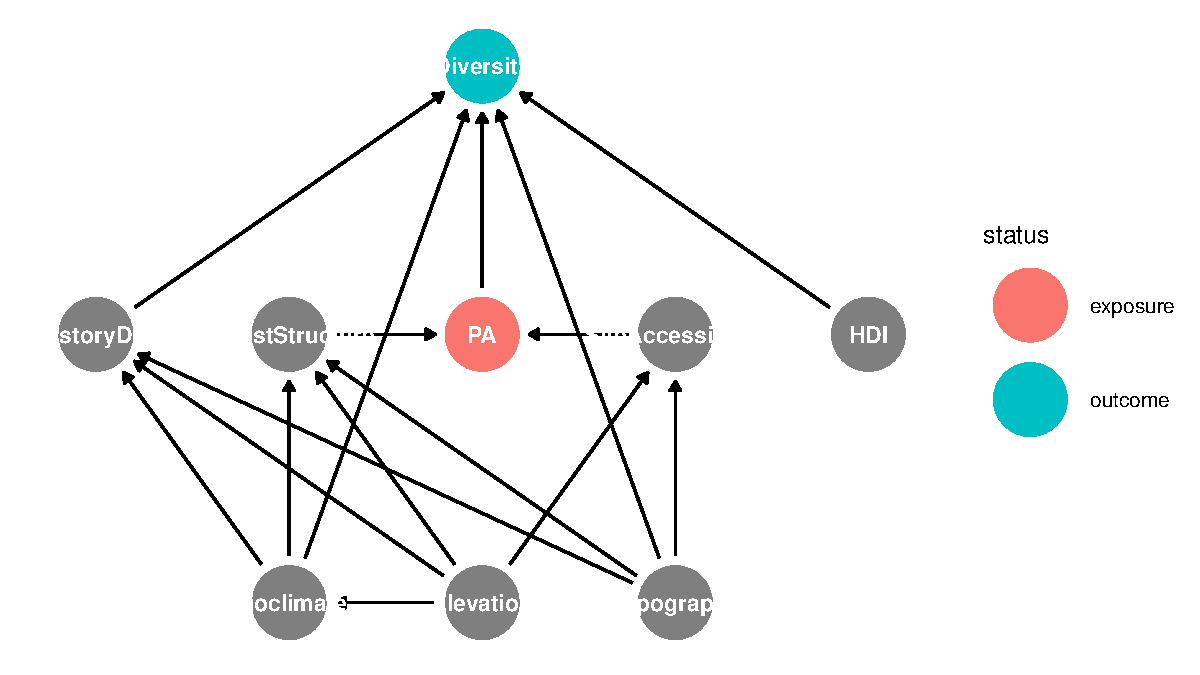
\includegraphics[width=576px]{/Users/wenxinyang/Desktop/GitHub/RPl-Brodie-2023/results/figures/1_scm-1}

\begin{Shaded}
\begin{Highlighting}[]
\CommentTok{\# Identify the set of adjustment variables needed to identify }
\CommentTok{\# the effect of PA on biodiversity and Test whether connectivity fulfills the }
\CommentTok{\# adjustment criterion}
\FunctionTok{adjustmentSets}\NormalTok{(dagBrodie)}
\end{Highlighting}
\end{Shaded}

\begin{verbatim}
## { Bioclimate, Topography, UnderstoryDensity }
## { Bioclimate, Elevation, Topography }
## { Elevation, ForestStructure, Topography }
## { ForestStructure, SiteAccessibility }
\end{verbatim}

\begin{Shaded}
\begin{Highlighting}[]
\CommentTok{\# isAdjustmentSet(dagBrodie, c("Connectivity"))}

\CommentTok{\# Plot the alternative adjustment sets}
\CommentTok{\# ggdag\_adjustment\_set(dagBrodie, }
\CommentTok{\#                      node\_size = 20, }
\CommentTok{\#                      text\_col = "black"}
\CommentTok{\# ) + ggplot2::theme(legend.position = "bottom")}
\end{Highlighting}
\end{Shaded}

\hypertarget{clean-protected-areas-might-take-a-while-to-run}{%
\subsubsection{Clean protected areas (might take a while to
run)}\label{clean-protected-areas-might-take-a-while-to-run}}

\begin{Shaded}
\begin{Highlighting}[]
\CommentTok{\# Load libraries, easy to switch to use groundhog}
\CommentTok{\# something wrong with the path in rmd {-}{-}\textgreater{} reset path}
\CommentTok{\# requires PhantomJS: webdriver::install\_phantomjs()}
\NormalTok{pkgs }\OtherTok{\textless{}{-}} \FunctionTok{c}\NormalTok{(}\StringTok{"sf"}\NormalTok{, }\StringTok{"dplyr"}\NormalTok{, }\StringTok{"terra"}\NormalTok{, }\StringTok{"optparse"}\NormalTok{, }\StringTok{"wdpar"}\NormalTok{, }\StringTok{"here"}\NormalTok{)}
\FunctionTok{sapply}\NormalTok{(pkgs, require, }\AttributeTok{character.only =} \ConstantTok{TRUE}\NormalTok{)}
\end{Highlighting}
\end{Shaded}

\begin{verbatim}
## Loading required package: sf
\end{verbatim}

\begin{verbatim}
## Warning: package 'sf' was built under R version 4.2.3
\end{verbatim}

\begin{verbatim}
## Linking to GEOS 3.11.0, GDAL 3.5.3, PROJ 9.1.0; sf_use_s2() is TRUE
\end{verbatim}

\begin{verbatim}
## Loading required package: terra
\end{verbatim}

\begin{verbatim}
## Warning: package 'terra' was built under R version 4.2.3
\end{verbatim}

\begin{verbatim}
## terra 1.7.65
\end{verbatim}

\begin{verbatim}
## Loading required package: optparse
\end{verbatim}

\begin{verbatim}
## Warning: package 'optparse' was built under R version 4.2.3
\end{verbatim}

\begin{verbatim}
## Loading required package: wdpar
\end{verbatim}

\begin{verbatim}
##       sf    dplyr    terra optparse    wdpar     here 
##     TRUE     TRUE     TRUE     TRUE     TRUE     TRUE
\end{verbatim}

\begin{Shaded}
\begin{Highlighting}[]
\FunctionTok{sf\_use\_s2}\NormalTok{(}\ConstantTok{FALSE}\NormalTok{) }\CommentTok{\# deal with buffering odd}
\end{Highlighting}
\end{Shaded}

\begin{verbatim}
## Spherical geometry (s2) switched off
\end{verbatim}

\begin{Shaded}
\begin{Highlighting}[]
\CommentTok{\# Command line inputs}
\NormalTok{option\_list }\OtherTok{\textless{}{-}} \FunctionTok{list}\NormalTok{(}
    \FunctionTok{make\_option}\NormalTok{(}\FunctionTok{c}\NormalTok{(}\StringTok{"{-}s"}\NormalTok{, }\StringTok{"{-}{-}src\_dir"}\NormalTok{), }
                \AttributeTok{action =} \StringTok{"store"}\NormalTok{, }\AttributeTok{default =} \StringTok{"data/raw/public"}\NormalTok{, }\AttributeTok{type =} \StringTok{\textquotesingle{}character\textquotesingle{}}\NormalTok{,}
                \AttributeTok{help =} \StringTok{"The source directory for reading data [default \%default]."}\NormalTok{),}
    \FunctionTok{make\_option}\NormalTok{(}\FunctionTok{c}\NormalTok{(}\StringTok{"{-}d"}\NormalTok{, }\StringTok{"{-}{-}dst\_dir"}\NormalTok{), }
                \AttributeTok{action =} \StringTok{"store"}\NormalTok{, }\AttributeTok{default =} \StringTok{\textquotesingle{}data/derived/public\textquotesingle{}}\NormalTok{, }\AttributeTok{type =} \StringTok{\textquotesingle{}character\textquotesingle{}}\NormalTok{,}
                \AttributeTok{help =} \FunctionTok{paste0}\NormalTok{(}\StringTok{"The path to save the csv [default \%default]."}\NormalTok{)))}
\NormalTok{opt }\OtherTok{\textless{}{-}} \FunctionTok{parse\_args}\NormalTok{(}\FunctionTok{OptionParser}\NormalTok{(}\AttributeTok{option\_list =}\NormalTok{ option\_list))}

\CommentTok{\# Directories and paths}
\NormalTok{src\_dir }\OtherTok{\textless{}{-}}\NormalTok{ opt}\SpecialCharTok{$}\NormalTok{src\_dir}
\NormalTok{dst\_dir }\OtherTok{\textless{}{-}}\NormalTok{ opt}\SpecialCharTok{$}\NormalTok{dst\_dir}

\CommentTok{\# Read samples and raster template}
\DocumentationTok{\#\# According to the pairs of lat/lon and east/north, they used}
\DocumentationTok{\#\# UTM Zone 46 (EPSG:32646) for projection, so here we will use the same one.}
\DocumentationTok{\#\# (Not mean it is the most right one to use)}
\NormalTok{fnames }\OtherTok{\textless{}{-}} \FunctionTok{list.files}\NormalTok{(}\FunctionTok{file.path}\NormalTok{(src\_dir, }\StringTok{"training"}\NormalTok{), }\AttributeTok{full.names =} \ConstantTok{TRUE}\NormalTok{)}
\FunctionTok{print}\NormalTok{(}\FunctionTok{file.path}\NormalTok{())}
\end{Highlighting}
\end{Shaded}

\begin{verbatim}
## character(0)
\end{verbatim}

\begin{Shaded}
\begin{Highlighting}[]
\NormalTok{pts }\OtherTok{\textless{}{-}} \FunctionTok{do.call}\NormalTok{(rbind, }\FunctionTok{lapply}\NormalTok{(fnames, }\ControlFlowTok{function}\NormalTok{(fname)\{}
    \FunctionTok{read.csv}\NormalTok{(fname) }\SpecialCharTok{\%\textgreater{}\%} 
        \FunctionTok{select}\NormalTok{(}\FunctionTok{all\_of}\NormalTok{(}\FunctionTok{names}\NormalTok{(.)[}
\NormalTok{            stringr}\SpecialCharTok{::}\FunctionTok{str\_detect}\NormalTok{(}\FunctionTok{names}\NormalTok{(.), }\StringTok{"station|country|lat|long"}\NormalTok{)])) }\SpecialCharTok{\%\textgreater{}\%} 
        \FunctionTok{st\_as\_sf}\NormalTok{(}\AttributeTok{coords =} \FunctionTok{c}\NormalTok{(}\DecValTok{3}\NormalTok{, }\DecValTok{2}\NormalTok{), }\AttributeTok{crs =} \DecValTok{4326}\NormalTok{)}
\NormalTok{\}))}

\NormalTok{template }\OtherTok{\textless{}{-}} \FunctionTok{rast}\NormalTok{(}
    \FunctionTok{file.path}\NormalTok{(src\_dir, }\StringTok{"GEDIv002\_20190417to20220413\_cover\_krig.tiff"}\NormalTok{)) }\SpecialCharTok{\%\textgreater{}\%} 
    \FunctionTok{extend}\NormalTok{(}\FunctionTok{c}\NormalTok{(}\DecValTok{100}\NormalTok{, }\DecValTok{100}\NormalTok{)) }\CommentTok{\# add a buffer}
\FunctionTok{values}\NormalTok{(template) }\OtherTok{\textless{}{-}} \DecValTok{1}\SpecialCharTok{:}\FunctionTok{ncell}\NormalTok{(template)}

\DocumentationTok{\#\#\#\#\#\#\#\#\#\#\#\#\#\#\#\#\#\#\#\#\#\#\#\#\#\# Query Protected areas (PAs) \#\#\#\#\#\#\#\#\#\#\#\#\#\#\#\#\#\#\#\#\#\#\#\#\#}
\DocumentationTok{\#\# Within this part, most of the issues related to PAs are solved }
\DocumentationTok{\#\# 1. Project the PAs or relevant layers to use precise distance.}
\DocumentationTok{\#\# 2. Trim the PAs to terrestrial only.}
\DocumentationTok{\#\# 3. Separate or union polygons and re{-}index them.}

\CommentTok{\# Query and clean PAs}
\CommentTok{\# skip these unless comments removed}
\CommentTok{\#raw\_pas \textless{}{-} c("KHM", "CHN", "IDN", "LAO", "MYS", }
\CommentTok{\#             "SGP", "THA", "VNM", "BRN") \%\textgreater{}\%}
\CommentTok{\#    lapply(wdpa\_fetch, wait = TRUE,}
\CommentTok{\#           download\_dir = rappdirs::user\_data\_dir("wdpar")) \%\textgreater{}\%}
\CommentTok{\#    bind\_rows()}
\CommentTok{\#raw\_pas \textless{}{-} wdpa\_clean(raw\_pas, crs = "EPSG:32646",}
\CommentTok{\#                      geometry\_precision = 100000)}
\CommentTok{\#raw\_pas \textless{}{-} raw\_pas \%\textgreater{}\% filter(MARINE != "marine")}
\DocumentationTok{\#\# Note: now the No is 1638}

\CommentTok{\# Trim the polygons to terrestrial only}
\DocumentationTok{\#\# Clip all not marine polygons to administrative border.}
\DocumentationTok{\#\# Use the same data source in examples of R package wdpar.}
\CommentTok{\# still skip this}

\CommentTok{\#raw\_adm\_bry \textless{}{-} lapply(}
\CommentTok{\#    c("KHM", "CHN", "IDN", "LAO", "MYS", }
\CommentTok{\#      "SGP", "THA", "VNM", "BRN"), function(iso)\{}
\CommentTok{\#          file\_path \textless{}{-} tempfile(fileext = "rds")}
\CommentTok{\#          lk \textless{}{-} "https://biogeo.ucdavis.edu/data/gadm3.6/Rsf"}
\CommentTok{\#          download.file(sprintf("\%s/gadm36\_\%s\_0\_sf.rds", lk, iso), file\_path)}
\CommentTok{\#          readRDS(file\_path)\}) \%\textgreater{}\% bind\_rows()}

\DocumentationTok{\#\# Process the boundary a bit}
\CommentTok{\# skipping}
\CommentTok{\#adm\_bry \textless{}{-} raw\_adm\_bry \%\textgreater{}\%}
\CommentTok{\#    st\_set\_precision(100000) \%\textgreater{}\%}
\CommentTok{\#    sf::st\_make\_valid() \%\textgreater{}\%}
\CommentTok{\#    st\_set\_precision(100000) \%\textgreater{}\%}
\CommentTok{\#    st\_combine() \%\textgreater{}\%}
\CommentTok{\#    st\_union() \%\textgreater{}\%}
\CommentTok{\#    st\_set\_precision(100000) \%\textgreater{}\%}
\CommentTok{\#    sf::st\_make\_valid() \%\textgreater{}\%}
\CommentTok{\#    st\_transform(st\_crs(raw\_pas)) \%\textgreater{}\%}
\CommentTok{\#    sf::st\_make\_valid()}

\DocumentationTok{\#\# Clip it to boundary}
\CommentTok{\# skipping}

\CommentTok{\#clean\_pas \textless{}{-} raw\_pas \%\textgreater{}\% st\_intersection(adm\_bry)}
\DocumentationTok{\#\# No of PAs drop from 1638 to 1618}

\CommentTok{\# Crop it to extent}
\CommentTok{\# skipping}
\DocumentationTok{\#\# }\AlertTok{WARNING}\DocumentationTok{: remember to re{-}run this step again after union/separate the polygons}

\CommentTok{\#bbox \textless{}{-} st\_as\_sfc(st\_bbox(template)) \%\textgreater{}\% st\_transform(st\_crs(clean\_pas))}
\CommentTok{\#clean\_pas \textless{}{-} clean\_pas \%\textgreater{}\% }
\CommentTok{\#    slice(unique(unlist(suppressMessages(st\_intersects(bbox, .)))))}
\DocumentationTok{\#\# Note: No of PAs drop further to 1260}

\CommentTok{\# Union/separate polygons.}
\CommentTok{\# Have to drop the attributes. Shouldn\textquotesingle{}t be a problem though.}
\CommentTok{\# skipping}

\CommentTok{\#clean\_pas \textless{}{-} st\_cast(st\_union(clean\_pas), "POLYGON") \%\textgreater{}\% }
\CommentTok{\#    st\_as\_sf() \%\textgreater{}\% rename(geometry = x)}
\DocumentationTok{\#\# No of PAs change from 1260 to 4270 (lose administrative meaning)}

\CommentTok{\# Crop to extent again}
\CommentTok{\# skipping}

\CommentTok{\#clean\_pas \textless{}{-} clean\_pas \%\textgreater{}\% }
\CommentTok{\#    slice(unique(unlist(suppressMessages(st\_intersects(bbox, .))))) \%\textgreater{}\% }
\CommentTok{\#    mutate(index = 1:nrow(.))}
\DocumentationTok{\#\# No of PAs change from 4270 to 4259}

\CommentTok{\# Re{-}calculate the area}
\CommentTok{\# skipping}

\CommentTok{\#clean\_pas \textless{}{-} clean\_pas \%\textgreater{}\% }
\CommentTok{\#    mutate(REP\_AREA = st\_area(.) \%\textgreater{}\% units::set\_units("km2"))}

\CommentTok{\# Clean the tiny ones with "partial" marine type due to a high chance to be the}
\CommentTok{\# noisy remaining of the clip}
\CommentTok{\# skipping}

\CommentTok{\#false\_pas \textless{}{-} st\_join(clean\_pas, raw\_pas \%\textgreater{}\% select(MARINE)) \%\textgreater{}\% }
\CommentTok{\#    filter(MARINE != "terrestrial" \& REP\_AREA \textless{} 0.01 \%\textgreater{}\% units::set\_units("km2"))}

\CommentTok{\#clean\_pas \textless{}{-} clean\_pas \%\textgreater{}\% filter(!index \%in\% unique(false\_pas$index))}

\DocumentationTok{\#\#\#\#\#\#\#\#\#\#\#\#\#\#\#\#\#\#\#\#\#\#\#\#\# Cluster Protected areas (PAs) \#\#\#\#\#\#\#\#\#\#\#\#\#\#\#\#\#\#\#\#\#\#\#\#}
\DocumentationTok{\#\# 4. Cluster the PAs that are connected. }
\DocumentationTok{\#\# The assumption here is that it is difficult (if not possible) for mammals }
\DocumentationTok{\#\# to pass the ocean or huge waterbodies.}
\DocumentationTok{\#\# Warning: this is only for mammal species}
\CommentTok{\# skipping}

\CommentTok{\#adm\_reorg \textless{}{-} raw\_adm\_bry \%\textgreater{}\% }
\CommentTok{\#    st\_transform(st\_crs(clean\_pas)) \%\textgreater{}\% }
\CommentTok{\#    st\_buffer(10) \%\textgreater{}\% st\_union() \%\textgreater{}\% st\_buffer({-}10) \%\textgreater{}\% st\_cast("POLYGON") \%\textgreater{}\% }
\CommentTok{\#    st\_intersection(bbox) \%\textgreater{}\% st\_as\_sf() \%\textgreater{}\% mutate(group = 1:nrow(.)) \%\textgreater{}\% }
\CommentTok{\#    mutate(area = st\_area(.) \%\textgreater{}\% units::set\_units("km2"))}

\CommentTok{\#clean\_pas \textless{}{-} st\_join(clean\_pas, adm\_reorg) \# No is 2873}

\DocumentationTok{\#\# Clean further}
\CommentTok{\# skipping}
\CommentTok{\#false\_pas \textless{}{-} clean\_pas \%\textgreater{}\% }
\CommentTok{\#    filter(area \textgreater{} 5e+05 \%\textgreater{}\% units::set\_units("km2") \& }
\CommentTok{\#               REP\_AREA \textless{} 1 \%\textgreater{}\% units::set\_units("km2"))}
\CommentTok{\#clean\_pas \textless{}{-} clean\_pas \%\textgreater{}\% filter(!index \%in\% unique(false\_pas$index)) \# 2198}

\DocumentationTok{\#\# Re{-}index}
\CommentTok{\# skipping}
\CommentTok{\#clean\_pas \textless{}{-} clean\_pas \%\textgreater{}\% mutate(index = 1:nrow(.)) \%\textgreater{}\% }
\CommentTok{\#    select({-}area)}

\CommentTok{\#adm\_reorg \textless{}{-} adm\_reorg \%\textgreater{}\% filter(group \%in\% clean\_pas$group) \%\textgreater{}\% }
\CommentTok{\#    rename(geometry = x) \%\textgreater{}\% select(group)}

\CommentTok{\# Save out}
\CommentTok{\# skipping and reading existing ones}
\CommentTok{\# st\_write(clean\_pas, file.path(dst\_dir, "clean\_pas.geojson"))}
\CommentTok{\# st\_write(adm\_reorg, file.path(dst\_dir, "pa\_groups.shp"))}

\NormalTok{clean\_pas }\OtherTok{\textless{}{-}} \FunctionTok{st\_read}\NormalTok{(}\FunctionTok{file.path}\NormalTok{(dst\_dir, }\StringTok{\textquotesingle{}clean\_pas.geojson\textquotesingle{}}\NormalTok{))}
\end{Highlighting}
\end{Shaded}

\begin{verbatim}
## Reading layer `clean_pas' from data source 
##   `/Users/wenxinyang/Desktop/GitHub/RPl-Brodie-2023/data/derived/public/clean_pas.geojson' 
##   using driver `GeoJSON'
## Simple feature collection with 2198 features and 3 fields
## Geometry type: POLYGON
## Dimension:     XY
## Bounding box:  xmin: 745225 ymin: -840825 xmax: 3601414 ymax: 2894781
## Projected CRS: WGS 84 / UTM zone 46N
\end{verbatim}

\begin{Shaded}
\begin{Highlighting}[]
\NormalTok{adm\_reorg }\OtherTok{\textless{}{-}} \FunctionTok{file.path}\NormalTok{(dst\_dir, }\StringTok{\textquotesingle{}pa\_groups.shp\textquotesingle{}}\NormalTok{)}
\end{Highlighting}
\end{Shaded}

\hypertarget{data-preparation-for-bird-models}{%
\subsubsection{Data preparation for bird
models}\label{data-preparation-for-bird-models}}

We first prepare data for the causal models for birds.

\begin{Shaded}
\begin{Highlighting}[]
\CommentTok{\# rm(list = ls())}

\CommentTok{\# Load the data provided by Brodie et al. (2023)}
\NormalTok{dat\_brodie\_bird }\OtherTok{\textless{}{-}} \FunctionTok{data.frame}\NormalTok{(}\FunctionTok{read.csv}\NormalTok{(}
                          \FunctionTok{here}\NormalTok{(}\StringTok{"data/raw/public/training/bird\_data\_230326.csv"}\NormalTok{), }
                          \AttributeTok{header =}\NormalTok{ T))}

\CommentTok{\# Simplify the variable names of site identifier and geographic coordinates}
\FunctionTok{names}\NormalTok{(dat\_brodie\_bird)[}\FunctionTok{names}\NormalTok{(dat\_brodie\_bird) }\SpecialCharTok{==} \StringTok{"site"}\NormalTok{] }\OtherTok{\textless{}{-}} \StringTok{"station"}
\FunctionTok{names}\NormalTok{(dat\_brodie\_bird)[}\FunctionTok{names}\NormalTok{(dat\_brodie\_bird) }\SpecialCharTok{==} \StringTok{"lat\_wgs84"}\NormalTok{] }\OtherTok{\textless{}{-}} \StringTok{"lat"}
\FunctionTok{names}\NormalTok{(dat\_brodie\_bird)[}\FunctionTok{names}\NormalTok{(dat\_brodie\_bird) }\SpecialCharTok{==} \StringTok{"long\_wgs84"}\NormalTok{] }\OtherTok{\textless{}{-}} \StringTok{"long"}

\CommentTok{\# Search for HDI in the column names }
\FunctionTok{grep}\NormalTok{(}\StringTok{"hdi"}\NormalTok{, }\FunctionTok{names}\NormalTok{(dat\_brodie\_bird), }\AttributeTok{value =} \ConstantTok{TRUE}\NormalTok{)}
\end{Highlighting}
\end{Shaded}

\begin{verbatim}
## character(0)
\end{verbatim}

\begin{Shaded}
\begin{Highlighting}[]
\FunctionTok{grep}\NormalTok{(}\StringTok{"HDI"}\NormalTok{, }\FunctionTok{names}\NormalTok{(dat\_brodie\_bird), }\AttributeTok{value =} \ConstantTok{TRUE}\NormalTok{)}
\end{Highlighting}
\end{Shaded}

\begin{verbatim}
## character(0)
\end{verbatim}

\begin{Shaded}
\begin{Highlighting}[]
\CommentTok{\# Assign stations the HDI value of its country}
\CommentTok{\# Reference: Human Development Report 2020: The Next Frontier—Human Development }
\CommentTok{\# and the Anthropocene (United Nations Development Programme, 2020).}
\CommentTok{\# https://hdr.undp.org/data{-}center/human{-}development{-}index\#/indicies/HDI}
\CommentTok{\# https://hdr.undp.org/sites/default/files/2021{-}22\_HDR/HDR21{-}22\_Statistical\_Annex\_HDI\_Table.xlsx}

\NormalTok{dat\_HDI }\OtherTok{\textless{}{-}} \FunctionTok{data.frame}\NormalTok{(}
    \AttributeTok{country =} \FunctionTok{unique}\NormalTok{(dat\_brodie\_bird}\SpecialCharTok{$}\NormalTok{country), }
    \AttributeTok{HDI =} \FunctionTok{c}\NormalTok{(}\FloatTok{0.593}\NormalTok{, }\FloatTok{0.768}\NormalTok{, }\FloatTok{0.705}\NormalTok{, }\FloatTok{0.607}\NormalTok{, }\FloatTok{0.803}\NormalTok{, }\FloatTok{0.939}\NormalTok{, }\FloatTok{0.800}\NormalTok{, }
            \FloatTok{0.703}\NormalTok{, }\FloatTok{0.829}\NormalTok{))}
\NormalTok{dat\_brodie\_bird }\OtherTok{\textless{}{-}} \FunctionTok{left\_join}\NormalTok{(dat\_brodie\_bird, dat\_HDI, }\AttributeTok{by =} \StringTok{"country"}\NormalTok{)}

\CommentTok{\# Create dataframe containing the subset of variable used in the analysis}
\NormalTok{dat\_bird }\OtherTok{\textless{}{-}}\NormalTok{ dat\_brodie\_bird }\SpecialCharTok{\%\textgreater{}\%} \FunctionTok{select}\NormalTok{(station, country, PA, utm\_east, utm\_north, }
\NormalTok{                             Hansen\_recentloss,access\_log10, HDI, dist\_to\_PA, }
\NormalTok{                             PA\_size\_km2, rh\_95\_a0.pred, pavd\_0\_5.pred, }
\NormalTok{                             pai\_a0.pred, fhd\_pai\_1m\_a0.pred, cover\_a0.pred, }
\NormalTok{                             agbd\_a0.pred,asymptPD, maxFRic, SR.mean)}

\CommentTok{\# Add the connectivity variables for each station calculated with }
\CommentTok{\# calc\_conn\_metrics.R}
\NormalTok{dat\_conn\_metrics\_bird }\OtherTok{\textless{}{-}} \FunctionTok{data.frame}\NormalTok{(}\FunctionTok{read.csv}\NormalTok{(}
                                \FunctionTok{here}\NormalTok{(}\StringTok{"data/derived/public/conn\_flux\_bird\_10\_150.csv"}\NormalTok{), }
                                \AttributeTok{header =}\NormalTok{ T))}
\NormalTok{dat\_bird }\OtherTok{\textless{}{-}} \FunctionTok{left\_join}\NormalTok{(dat\_bird, dat\_conn\_metrics\_bird, }\AttributeTok{by =} \StringTok{"station"}\NormalTok{)}

\CommentTok{\# Scale subset of continuous variables in dat}
\CommentTok{\# Peter {-} Need to add the connectivity measures to the scaling list when they }
\CommentTok{\# are introduced}
\NormalTok{dat\_scale\_bird }\OtherTok{\textless{}{-}} \FunctionTok{data.frame}\NormalTok{(}\FunctionTok{scale}\NormalTok{(}\FunctionTok{subset}\NormalTok{(dat\_bird, }\AttributeTok{select =} \FunctionTok{c}\NormalTok{(}\StringTok{"utm\_east"}\NormalTok{, }\StringTok{"utm\_north"}\NormalTok{, }
                                                     \StringTok{"HDI"}\NormalTok{, }\StringTok{"access\_log10"}\NormalTok{, }
                                                     \StringTok{"PA\_size\_km2"}\NormalTok{, }
                                                     \StringTok{"dist\_to\_PA"}\NormalTok{, }
                                                     \StringTok{"rh\_95\_a0.pred"}\NormalTok{, }
                                                     \StringTok{"pavd\_0\_5.pred"}\NormalTok{, }
                                                     \StringTok{"pai\_a0.pred"}\NormalTok{, }
                                                     \StringTok{"fhd\_pai\_1m\_a0.pred"}\NormalTok{, }
                                                     \StringTok{"cover\_a0.pred"}\NormalTok{, }
                                                     \StringTok{"agbd\_a0.pred"}\NormalTok{,}
                                                     \StringTok{"awf\_ptg"}\NormalTok{), }
\NormalTok{                                     ), }
                              \AttributeTok{center =} \ConstantTok{TRUE}\NormalTok{, }\AttributeTok{scale =} \ConstantTok{TRUE}\NormalTok{))}

\CommentTok{\# Append scaled variables to data with .z suffixes}
\NormalTok{dat\_bird[}\FunctionTok{paste0}\NormalTok{(}\FunctionTok{names}\NormalTok{(dat\_scale\_bird), }\StringTok{\textquotesingle{}.z\textquotesingle{}}\NormalTok{)] }\OtherTok{\textless{}{-}}\NormalTok{ dat\_scale\_bird}

\CommentTok{\# Rename scaled, predicted relative canopy height at 95\% (rh\_95\_a0.pred.z) }
\CommentTok{\# as forest\_structure to match DAG }
\FunctionTok{names}\NormalTok{(dat\_bird)[}\FunctionTok{names}\NormalTok{(dat\_bird) }\SpecialCharTok{==} \StringTok{"rh\_95\_a0.pred.z"}\NormalTok{] }\OtherTok{\textless{}{-}} \StringTok{"forest\_structure"}

\CommentTok{\# Rename scaled, predicted plant area volume density between 0m and 5m }
\CommentTok{\# (pavd\_0\_5.pred.z) as understory\_density to match DAG}
\FunctionTok{names}\NormalTok{(dat\_bird)[}\FunctionTok{names}\NormalTok{(dat\_bird) }\SpecialCharTok{==} \StringTok{"pavd\_0\_5.pred.z"}\NormalTok{] }\OtherTok{\textless{}{-}} \StringTok{"understory\_density"}

\CommentTok{\# Exclude stations that underwent recent forest loss as defined by }
\CommentTok{\# Hansen et al. (2013)}
\NormalTok{dat\_clean\_bird }\OtherTok{\textless{}{-}} \FunctionTok{subset}\NormalTok{(dat\_bird, Hansen\_recentloss }\SpecialCharTok{==} \DecValTok{0}\NormalTok{)}
\end{Highlighting}
\end{Shaded}

\hypertarget{bird-models}{%
\subsubsection{Bird models}\label{bird-models}}

\begin{table}
\centering
\begin{tabular}[t]{lccc}
\toprule
  & (1) & (2) & (3)\\
\midrule
(Intercept) & \num{2.919} & \num{224.401} & \num{127.216}\\
 & (\num{0.222}) & (\num{9.953}) & (\num{11.862})\\
forest\_structure & \num{0.088} & \num{38.936} & \num{19.493}\\
 & (\num{0.032}) & (\num{2.812}) & (\num{2.095})\\
access\_log10.z & \num{-0.090} & \num{7.804} & \num{10.956}\\
 & (\num{0.023}) & (\num{2.257}) & (\num{1.604})\\
HDI.z & \num{-0.011} & \num{-13.494} & \num{-7.122}\\
 & (\num{0.170}) & (\num{7.405}) & (\num{9.257})\\
PA & \num{0.370} & \num{13.501} & \num{30.511}\\
 & (\num{0.076}) & (\num{6.207}) & (\num{4.811})\\
SD (Intercept country) & \num{0.530} & \num{19.948} & \num{29.960}\\
SD (Observations) & \num{1.012} & \num{75.813} & \num{59.710}\\
\midrule
Num.Obs. & \num{1100} & \num{1101} & \num{1099}\\
R2 Marg. & \num{0.047} & \num{0.225} & \num{0.166}\\
R2 Cond. & \num{0.252} &  & \\
AIC & \num{3874.5} & \num{13876.9} & \num{13435.1}\\
BIC & \num{3919.6} & \num{13921.9} & \num{13480.1}\\
ICC & \num{0.2} &  & \\
RMSE & \num{0.89} & \num{65.44} & \num{65.15}\\
\bottomrule
\end{tabular}
\end{table}

\hypertarget{data-preparation-for-mammal-models}{%
\subsubsection{Data preparation for mammal
models}\label{data-preparation-for-mammal-models}}

\hypertarget{model-running}{%
\subsubsection{Model running}\label{model-running}}

\hypertarget{results}{%
\section{Results}\label{results}}

Describe how results are to be presented.

\hypertarget{discussion}{%
\section{Discussion}\label{discussion}}

Describe how the results are to be interpreted \emph{vis a vis} each
hypothesis or research question.

\hypertarget{integrity-statement}{%
\section{Integrity Statement}\label{integrity-statement}}

Include an integrity statement - The authors of this preregistration
state that they completed this preregistration to the best of their
knowledge and that no other preregistration exists pertaining to the
same hypotheses and research. If a prior registration \emph{does} exist,
explain the rationale for revising the registration here.

\hypertarget{acknowledgements}{%
\section{Acknowledgements}\label{acknowledgements}}

\begin{itemize}
\tightlist
\item
  \texttt{Funding\ Name}: name of funding for the project
\item
  \texttt{Funding\ Title}: title of project grant
\item
  \texttt{Award\ info\ URI}: web address for award information
\item
  \texttt{Award\ number}: award number
\end{itemize}

This report is based upon the template for Reproducible and Replicable
Research in Human-Environment and Geographical Sciences,
\url{DOI:\%5B10.17605/OSF.IO/W29MQ}{]}(\url{https://doi.org/10.17605/OSF.IO/W29MQ})

\hypertarget{references}{%
\section{References}\label{references}}

\end{document}
